
\begin{table*}[t!]
    \centering
    % Paired t-test Results Table
    \begin{tabular}{llcccccc}
    \toprule
    \multirow{2}{*}{Metric} & \multirow{2}{*}{Alt. Hyp.} & \multicolumn{6}{c}{Temperature} \\
    \cmidrule(lr){3-8}
    & & \multicolumn{2}{c}{$\tau=1.0$} & \multicolumn{2}{c}{$\tau=2.0$} & \multicolumn{2}{c}{$\tau=3.0$} \\
    \cmidrule(lr){3-4} \cmidrule(lr){5-6} \cmidrule(lr){7-8}
    & & $t$ & $p$ & $t$ & $p$ & $t$ & $p$ \\
    \midrule
    \multirow{2}{*}{Quality} & \texttt{Min-p} $>$ \texttt{Basic} & 0.33 & .370 & 0.65 & .260 & 3.13$^{***\dagger}$ & .001 \\
    & \texttt{Min-p} $>$ \texttt{Top-p} & 2.05$^{*}$ & .023 & 1.18 & .121 & 2.02$^{*}$ & .025 \\
    \midrule
    \multirow{2}{*}{Diversity} & \texttt{Min-p} $>$ \texttt{Basic} & 0.31 & .378 & 1.86$^{*}$ & .034 & 0.85 & .201 \\
    & \texttt{Min-p} $>$ \texttt{Top-p} & 2.64$^{**}$ & .006 & 1.44 & .078 & 0.87 & .195 \\
    \bottomrule
    \multicolumn{8}{l}{\scriptsize{$^{*}$ $p < 0.05$, $^{**}$ $p < 0.01$, $^{***}$ $p < 0.001$, $^{\dagger}$ Significant after Bonferroni correction for 12 comparisons.}} \\
    \multicolumn{8}{l}{\scriptsize{Note: All tests were paired t-tests with df = 52, one-sided (alternative = "greater")}} \\
    \phantom{Blank Line}\\
    \end{tabular}\\
    \captionof{table}{\textbf{Corrected Statistical Hypothesis Testing of Human Evaluators' Scores Fails to Support Claim that \texttt{Min-p} Consistently Outperforms Other Samplers.} To test whether evidence supports the claim that \texttt{min-p} ``consistently outperforms" other samplers, we conducted one-sided paired t-tests using the authors' published data. Without correcting for multiple comparisons, evidence supports \texttt{min-p}'s superiority in 5 of 12 comparisons at $\alpha=0.05$ and 2 of 12 comparisons at $\alpha=0.01$. After applying a Bonferroni correcting for multiple comparisons, evidence supports \texttt{min-p}'s superiority in 1 of 12 comparisons at $\alpha=0.05$ and 0 of 12 comparisons at $\alpha=0.01$..}
    \label{tab:human_evals_paired_ttests}
\end{table*}



\section{Standard 2: Valid Statistical Inference}


We next discuss critical issues regarding invalid statistical inference.
To rectify the record, we demonstrate a concrete statistical framework (Intersection-Union Test, Bonferroni correction) necessary for claiming ``consistent'' superiority, and show how it finds no statistically significant evidence to support \texttt{min-p}'s superiority.

We focus on \citet{nguyen2024minp}'s human evaluations, since human judgments are widely considered the gold standard for assessing language models \citep{van2019best,roller2020opendomainconversationalagentscurrent,howcroft2020twenty,clark2021all,liang2022holistic,khashabi2022geniereproduciblestandardizedhuman,chiang2024chatbotarenaopenplatform,biderman2024lessonstrenchesreproducibleevaluation,schaeffer2025correlatingpredictinghumanevaluations}, but emphasize that machine learning research involving human evaluations are frequently laden with statistical flaws \citep{freitag2021experts,belz2021reprogen,thomson2024common}.
This highlights how pervasive these issues can be.

To briefly explain the human evaluation methodology, three samplers (\texttt{basic}, \texttt{top-p} and \texttt{min-p}) were compared in six conditions: three temperatures ($1.0, 2.0, 3.0$) and two diversity settings (``high" and ``low") corresponding to different $p$ hyperparameters.
Humans were asked to score the generated outputs under two metrics: quality and diversity.
Participants were excluded if they failed attention checks.
For more information, please see the original manuscript.

\paragraph{Incorrect Data Pooling in Statistical Inference}

The original paper concluded that \texttt{min-p} ``consistently outperformed \texttt{top-p} across all settings'' based on a paired t-test that yielded $p<0.05$.
However, this statistical analysis reached an incorrect conclusion due to invalid statistical inference: despite claiming consistency across all metrics, temperatures, and diversity settings, the paper pooled data across all conditions to perform a single test.
This approach merely tests whether \texttt{min-p} scored higher on average, rather than consistently.
Furthermore, pooling was misleading because \texttt{top-p}'s p hyperparameter was poorly chosen in the ``low'' diversity condition ($p=0.1$), pulling its average down significantly, a condition the authors later publicly stated should be ignored.

\begin{figure*}[t!]
    \centering
    \begin{minipage}{\textwidth}
        \centering
        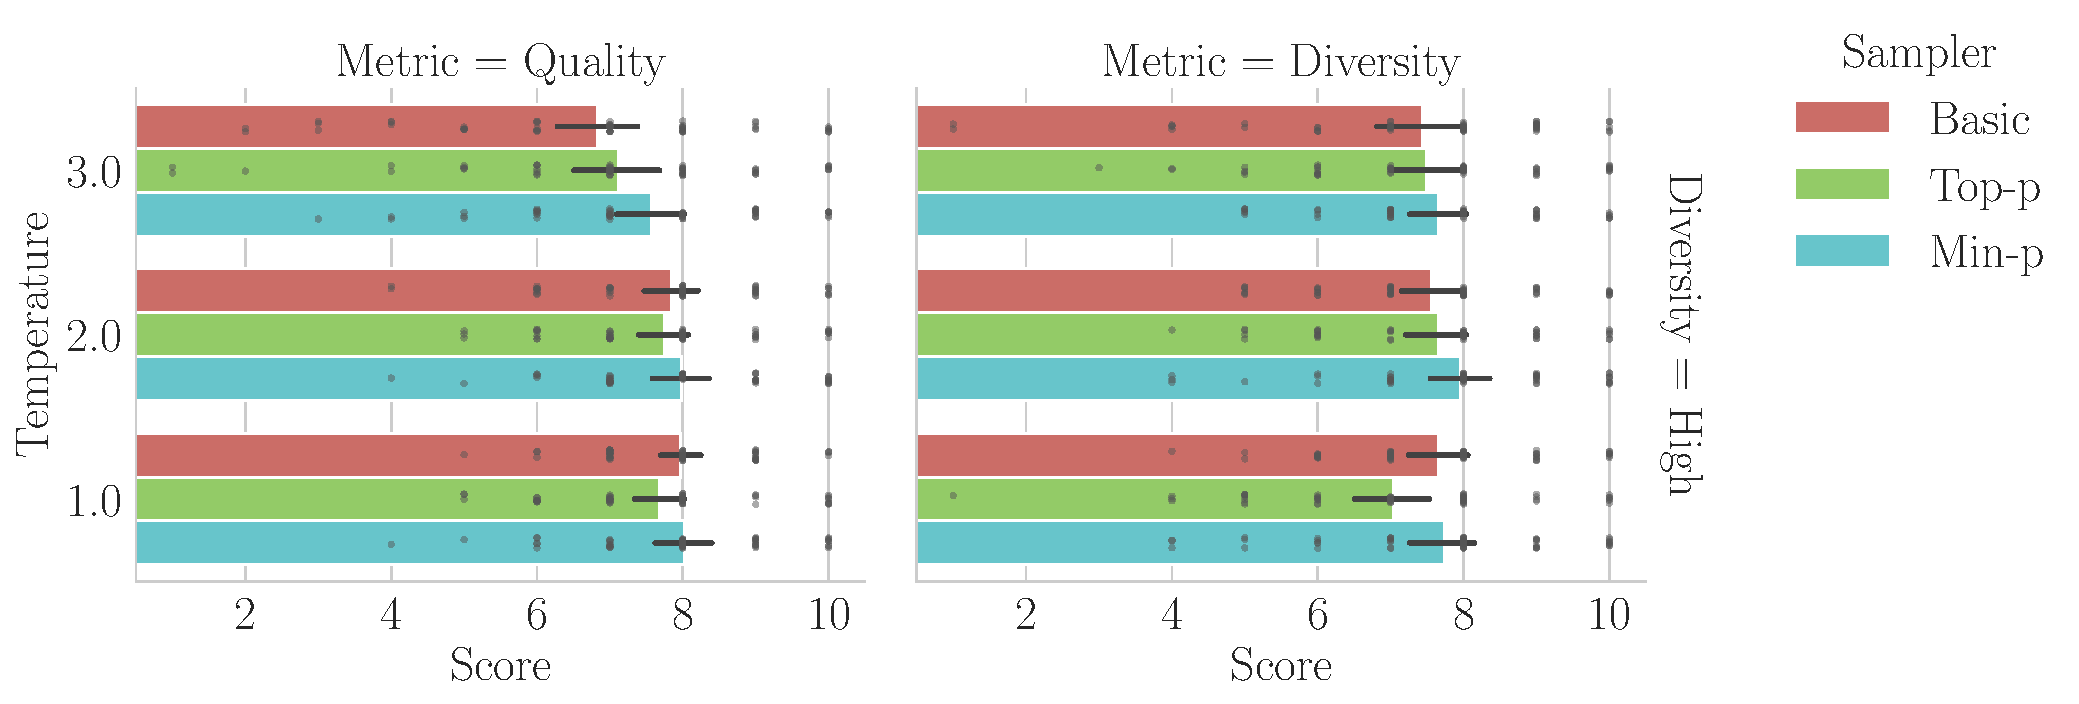
\includegraphics[width=\linewidth]{figures/human_evals/attentive_y=temp_x=score_hue=sampler_row=diversity_col=metric_barnstrip.pdf}
        \captionof{figure}{\textbf{Proper Visualization of of Human Evaluators' Scores Demonstrates \texttt{Min-p} Does Not ``Consistently" Outperform Other Samplers.} Visualization of human evaluators' scores from \citet{nguyen2024minp}'s first human experiment. Rather, the original paper's data suggest \texttt{min-p} is largely indistinguishable from other samplers based on 95\% confidence intervals.}
        \label{fig:human_evals}
    \end{minipage}
\end{figure*}


\begin{figure*}[t!]
    \centering
    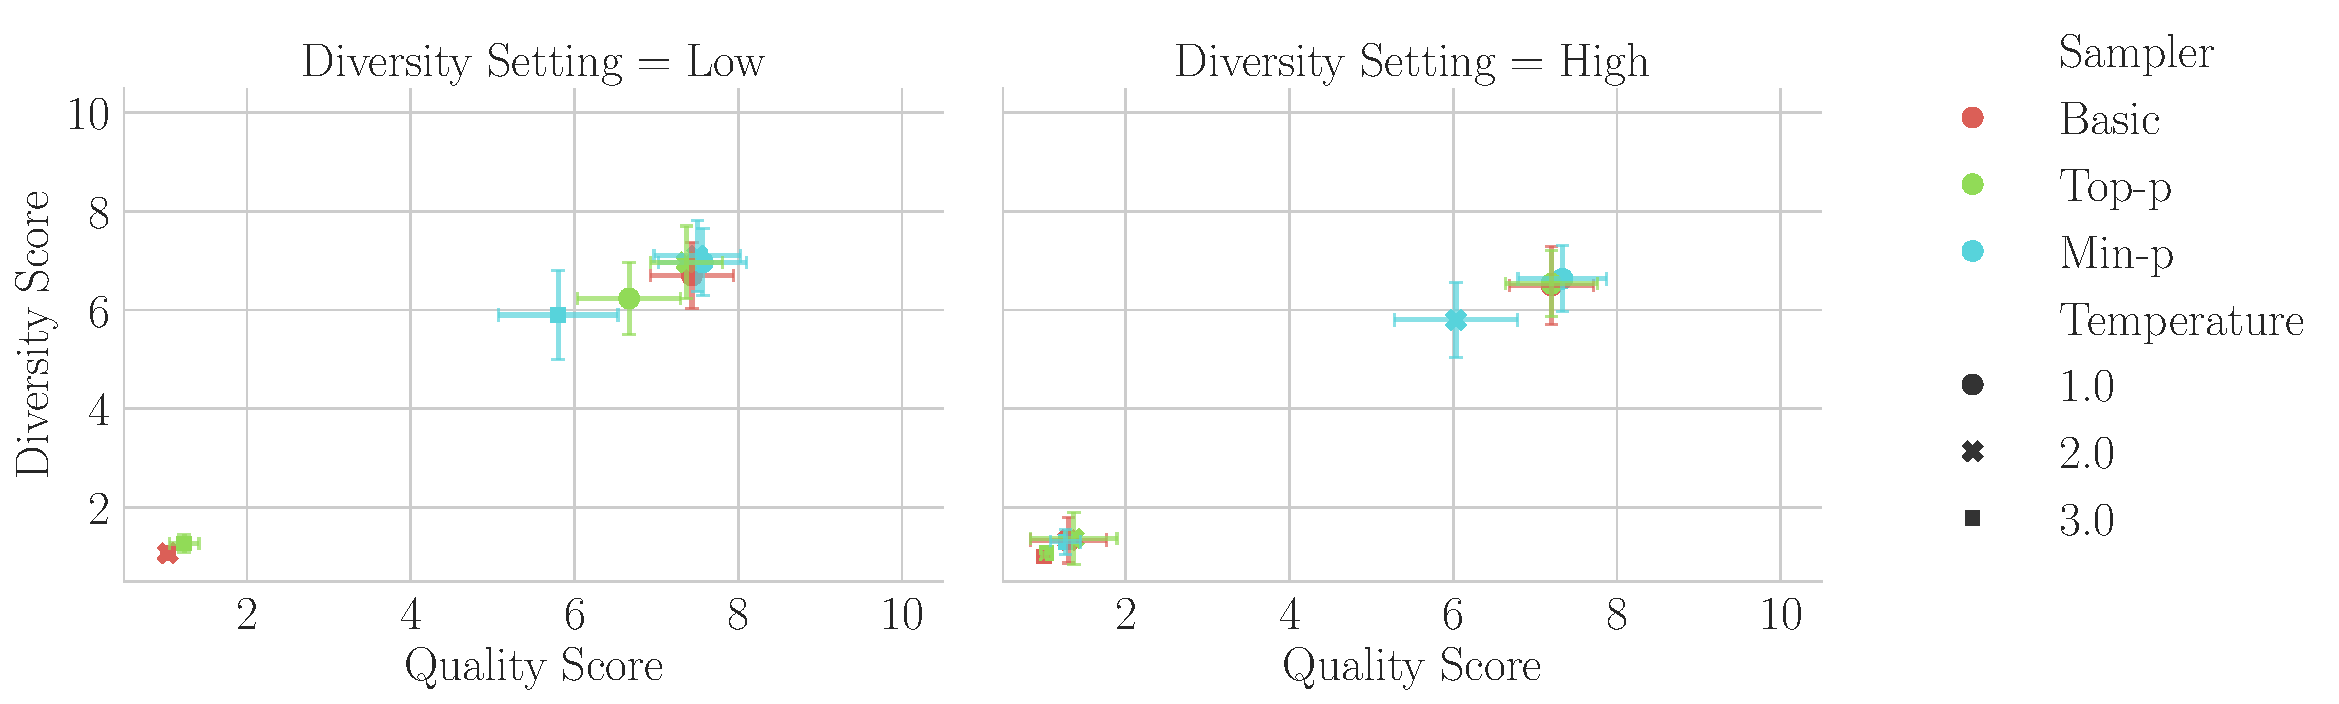
\includegraphics[width=\linewidth]{figures/new_human_evals/attentive_y=diversity_score_x=quality_score_hue=sampler_col=diversity_style=temp.pdf}
    \captionof{figure}{\textbf{Proper Visualization of Human Evaluators' Scores Suggests \texttt{Min-p} Does Not Outperform Baselines in Quality, in Diversity or in a Pareto-Optimal Tradeoff Between Quality and Diversity.} Visualization of human evaluators' scores from \citet{nguyen2024minp}'s second human experiment. These human evaluation results suggest that \texttt{min-p} offers no apparent advantage over \texttt{basic} sampling or \texttt{top-p} sampling.
    }
    \label{fig:new_human_evals}
\end{figure*}



\paragraph{Bonferroni Correction and Intersection-Union Test}



We focused on the ``high" diversity setting for three reasons: 
(1) The claimed advantage of \texttt{min-p} is that it provides both high quality and high diversity, whereas other samplers typically trade one against the other. (2) \href{https://github.com/menhguin/minp_paper/issues/4}{The authors publicly told us to focus on the high diversity setting}, writing, ``the low [diversity] settings were quite experimental.'' (3) We believe \texttt{top-p}'s $p$ hyperparameter in the low diversity setting was poorly chosen; indeed, after we raised said concerns, the authors ran a new human evaluation which changed the low diversity \texttt{top-p} $p$ from $0.1 \to 0.9$.


To more rigorously assess the claim that \texttt{min-p} consistently outperforms other samplers, we conducted 12 one-sided paired t-tests for each metric (quality or diversity), temperature ($1.0, 2.0, 3.0$) and baseline sampler (\texttt{min-p} versus \texttt{basic}, \texttt{min-p} versus \texttt{top-p}). In each test, the null hypothesis is \texttt{min-p}'s score is less than or equal to the other sampler's score, and the alternative hypothesis is \texttt{min-p}'s score is greater than the other sampler's score.
Statistical test results are displayed in Table~\ref{tab:human_evals_paired_ttests}.
Without correcting for multiple comparisons, we found evidence to reject the null hypotheses in 5 of 12 tests at $\alpha=0.05$ and 2 of 12 tests at $\alpha=0.01$. After applying a Bonferroni correction for multiple comparisons, we found evidence to reject the null hypothesis in 1 of 12 tests at $\alpha=0.05$ and 0 of 12 tests at $\alpha=0.01$.
Furthermore, given that the original paper claims that \texttt{min-p} ``consistently" scores higher, an Intersection-Union Test (IUT) may be the appropriate statistical test, where the alternative hypothesis is that \texttt{min-p} is better in all 12 comparisons and the null hypothesis is the set complement. Since the largest p-value of the 12 comparisons is $0.378$, under the IUT, we again find insufficient evidence to reject the null hypothesis at both $\alpha=0.05$ and $\alpha=0.01$.
\textbf{Based on the original paper's data, there is insufficient evidence to support the claim that \texttt{min-p} consistently outperforms baseline samplers across all settings.}



\paragraph{Proper Visualization of Evidence}

The lack of statistical significance is further reinforced by proper visualization. Using the original paper's data, Fig.~\ref{fig:human_evals} reveals that the three samplers provide similar quality and diversity, with 95\% confidence intervals frequently overlapping across temperatures. This visual evidence suggests \texttt{min-p} is largely indistinguishable from baselines in almost all settings.

When presented with these findings, the authors conducted and added a new human evaluation study.
Their new study made multiple methodological changes:
%
\begin{itemize}
    \item Different sampler implementation: switched from applying temperature \textit{after} truncation to applying temperature \textit{before} truncation.
    \item Different distribution of human participants from Prolific.
    \item Different hyperparameters for \texttt{top-p}: switched from $0.1$ and $0.9$ to $0.9$ and $0.95$.
    \item Different hyperparameters for \texttt{min-p}: switched from $0.2$ and $0.05$ to $0.1$ and $0.05$.
    \item Different allotted reading time: increased from 30 minutes to 45 minutes.
    \item Different sampled text: 3 short paragraphs were replaced with a single complete story.
    \item Different rubric for human participants to evaluate sampled outputs.
\end{itemize}
%
Regarding the \href{https://github.com/menhguin/minp_paper/blob/main/%5BLIVE%5D%20min_p%20user%20preference%20study%20v3.0%20(Responses)%20-%20Form%20responses%201.csv}{new human evaluation data} and results, we share two discoveries here:
First, more generally, the data show again that \texttt{min-p} does not outperform baseline sampling methods in quality, in diversity or in a favorable tradeoff between quality and diversity (Fig.~\ref{fig:new_human_evals}).
Second, we believe one value is incorrectly reported: in \citet{nguyen2024minp}'s Table 15, the average score of \texttt{min-p} at $p=0.05$ and temperature $T=2$ is reported as $7.80$, but based on the authors' publicly posted data, we believe the correct numerical value should be $5.80$. 
Both statistical hypothesis tests and proper visualizations of the human evaluation data suggest \texttt{min-p} is indistinguishable from the baselines in almost all settings.






%
% In this new study, whenever \texttt{min-p} outperforms other samplers, it does so under conditions that yield lower absolute scores than other conditions . For instance, \texttt{min-p} shows an advantage over the baselines in the ``high" diversity setting at $T=2$ and in the ``low" diversity setting at $T=3$. However, in both of these conditions, \texttt{min-p} receives lower quality and diversity scores than it does in the ``high" diversity setting at $T=1$ and the ``low" diversity setting at $T=2$. This shows \texttt{min-p}'s advantage is observed primarily under conditions that yield lower overall quality and diversity scores compared to other achievable conditions. 
% \textbf{For anyone seeking higher quality or diversity, \texttt{min-p} offers no apparent advantage over previously existing samplers}.
